\chapter{Implementation}
After providing an analysis of UIProtocol, settling down on the requirements and working out the design of the app, we can now present how the application was developed, what technologies were used, what problems were encountered and how they were tackled. It has been said that the app architecture was not influenced by any of the existing implementations. The client-server communication, however, was observed from another, already implemented client. Inspecting the communication logs helped to develop this client.

\subsection{Development Environment}
As previously said, the application was written in the Visual Studio 2013 IDE and using C\#, a programming language developed by Microsoft. The reasons for choosing Visual Studio (VS) are clear: VS is the main development tool for the whole .NET platform, fully supports C\# and Windows Phone development and debugging. VS is therefore the main tool to be used for most .NET development.

The programming was backed up by running the code directly on a Windows Phone 8 device, namely HTC 8S. We also used ReSharper, a useful plugin for code inspection, maintenance, refactoring and coding assistance.

\subsection{Overview of the Core Classes}
In this section, we will cover the most important classes of the application, to give a brief idea of how the UIP documents are handled, stored, processed and how the UI is rendered. There are several tables in the following pages, documenting classes for inner UIP Document representation (table \ref{tab:uipDocClasses}), rendering support (table \ref{tab:uipRenderClasses}), the communication with the server (table \ref{tab:uipCommClasses}) and the classes for management of interfaces and models (table \ref{tab:uipManagers}).

\begin{table}[htbp]
  \centering
  \caption{UIP Document Representation Classes}
  \label{tab:uipDocClasses}
 \renewcommand{\arraystretch}{1.2}
    \begin{tabularx}{\textwidth}{p{2.5cm}|X}
    \rowcolor{mygray}
    \textbf{Class Name} & \textbf{Class Description} \\
       Interface & This class represents the UIP interface as a container for more UI elements. This class has its own position, a container and can be embedded into another interface, as specified in Listing \ref{uipInterface}. \\ \hline
       Container & This is the class that stores the information about the particular UI elements. A Container can contain other Containers and instances of Element class.\\ \hline
       Element & Class representing particular UI elements such as button, textfield and more. \\
    \end{tabularx}%
    \label{tab:uipDocClasses2}
\end{table}%
\begin{table}[htbp]
  \centering
  \caption{UIP Server connection classes}
  \label{tab:uipCommClasses}
 \renewcommand{\arraystretch}{1.2}
    \begin{tabularx}{\textwidth}{p{3cm}|X}
    \rowcolor{mygray}
    \textbf{Class name} & \textbf{Class description} \\
      UipConnection & Initiates the connection and is responsible for sending events to the server and processing its responses. Does basic XML validation. \\ \hline
       SocketWorker & Handles the socket communication with UIP server. Sends events and runs a separate thread for receiving server's responses. \\ \hline
       HttpConncetion & Class responsible for acquiring resources via HTTP.
    \end{tabularx}%
\end{table}%
\begin{table}[htbp]
  \centering
  \caption{ModelManager and InterfaceManager classes}
  \label{tab:uipManagers}
 \renewcommand{\arraystretch}{1.2}
    \begin{tabularx}{\textwidth}{p{3cm}|X}
    \rowcolor{mygray}
    \textbf{Class name} & \textbf{Class description} \\
     ModelManager & Keeps and updates all requested and received models. Is implemented as a singleton class. \\ \hline
       \hspace{0pt}InterfaceManager & Stores all received interfaces. Provides getter method and method for rendering an \texttt{Interface}. Is also implemented as a singleton.\\
    \end{tabularx}%
\end{table}%


\subsection{Communication With UIP Server}
As shown in table \ref{tab:uipCommClasses}, the communication with server is implemented in \texttt{UipConnection} class which exposes its functionality for sending events to the rest of the application - namely the \texttt{EventManager} class. It also is responsible for processing any XML data received from the server. This data is forwarded to it from the \texttt{SocketWorker} instance.

\texttt{SocketWorker} is the low-level socket communication class which sends events to the server. It also runs an instance of \texttt{BackgroundWorker} class which, in an extra thread, awaits data from the server. The reason there is a separate thread for receiving data is that we cannot make any assumptions about when the server will send data to the client. Generally speaking, server can decide to send model updates at any time - not only as a response to a certain user action.

\subsection{Model Updates and Binding}
Any property of UIP document can, instead of direct value, contain a reference to a model and its property, as described in \ref{subsec:models}. As an example, let us consider a button. The text displayed in the button (its \texttt{Content}) can be either hard-coded into the UIP document or there can be a reference to a model property. If the reference is present, the \texttt{ModelManager} looks into an internally stored dictionary of models and if the model is present, the value of its corresponding property is immediately used. If that is not the case, \texttt{ModelManager} makes a request for the model and once it arrives, its corresponding property's value is used. In both cases, a binding is created so that the future updates of the model property are correctly propagated throughout the application. The \texttt{ModelManager} class only needs to be instantiated once, so that the application state is stored in one place. Therefore \texttt{ModelManager} is a singleton class.

The code which acquires the models and creates bindings between model properties and properties of UI elements makes heavy use of asynchronous methods. The async/await operations were introduced with C\# 5.0  and provide the developer with a comfortable way to deal with operations that are potentially blocking.

Because requesting and receiving models typically happens over a wireless connection, it can be considered potentially blocking. If a model request and its receiving was blocked within a synchronous process, the entire application would be forced to wait. However, by taking advantage of the asynchronous programming, the application continues with other work that does not depend on the web resource.

This is also the reason why sometimes the UI is drawn gradually. This happens when properties refer to models which have to be requested and received from the server - for example if a button text color is specified in a model. In such case, the button is rendered with the standard text color, and only once the model arrives, the font color is changed to whatever value is specified in the model. The delay before the update is noticeable but very short, and therefore does not limit the app usage in any way. The same happens to resources (images) from the HTTP server which are also fetched asynchronously.

\subsection{Interpolations (animations)}
Interpolation allows to move UI controls on the canvas. Because interpolation uses model updates, the prerequisite for it is that the UI control's coordinate which we want to change is bound to a model (e.g. if we want to move a button horizontally, we need to bind the \texttt{x} coordinate of its \texttt{Position} to a model property). It is triggered by an event which is fired by activating some UI control. The server responds by a model update whose body contains "interpolation" and "duration" attributes. An example of such model update is shown in listing \ref{uipInterpolation}.

\lstinputlisting[label=uipInterpolation,caption=UIP model update specifying interpolation]{sources/uipInterpolation.xml}

Interpolation works through model-wide binding. The \texttt{ModelManager}, when it receives an interpolation model, starts a new \texttt{Task} which periodically updates the given property value (property \texttt{x}, considering our example). Because of the data binding, this update also triggers update of the UI control's position on the canvas, which causes the UI control to move (animate).

\subsection{Binding Converters}
It has been said that any property can be bound to a model. However, properties in UIP document can convey a wide range of information - including color, font size, row and column position in a grid and etc. Since the model updates are always received as string, the binding has to be provided with a converter which, considering the given examples, converts the received string to \texttt{SolidColorBrush}, double and integer types, respectively. All of our converters implement \texttt{IValueConverter} interface, which is the standard way to apply custom logic to a binding.

\subsection{Implementing the UI Element Classes}
When deciding how to represent the platform native components which are displayed to the user, we chose to use wrapper classes which will expose the wrapped object's methods and at the same time be able to set up its properties from an instance of \texttt{Element} class (i.e. from the inner object representation).

All supported native components are therefore wrapped into other classes whose names indicate the enclosed UI element (e.g. \texttt{UipButton} is a wrapper class of the standard \texttt{Button} class). All of these wrapper classes inherit from abstract class \texttt{UipBase} which provides common support for model binding for all inherited components. This way, adding new UI components with binding support is made easy.

The \texttt{ITextStylable} interface is implemented by classes which contain text which can be styled. For example, a \texttt{UipTextBlock} implements this interface in order to be able to set font size, color and more. \texttt{UipPanel}, on the other hand, does not implement it because a container itself does not have any text to be styled.

The figure \ref{fig:UIclasses} shows a class diagram of a few wrapper classes and also \texttt{ITextStylable} being implemented.

\begin{figure}[ht!]
\centering
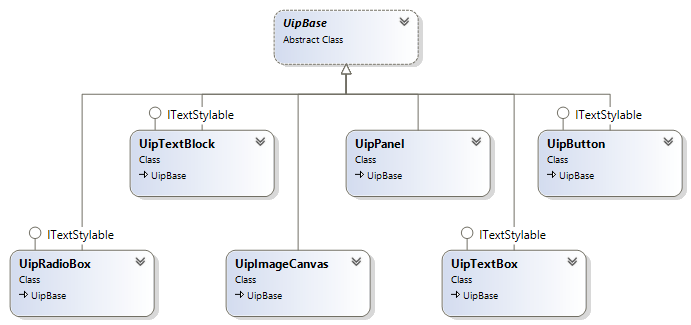
\includegraphics[width=140mm]{pics/UI_classes.png}
\caption{Inheritance tree of several sample UI classes}
\label{fig:UIclasses}
\end{figure}

\subsection{Rendering}
Rendering is always triggered by \texttt{InterfaceManager} class which calls the \texttt{Render()} method of \texttt{Renderer} class. Part of method body is shown in  listing \ref{uipRendering}. The method receives an \texttt{IRenderable item}  (i.e. instance of \texttt{Interface}, \texttt{Container} or \texttt{Element}) and a parent container. The method traverses the tree of UI elements, calling itself recursively if it encounters a container.

The foreach loop iterates over all elements in the container and creates a wrapper class for each of the \texttt{IRenderable}s. Note the graceful degradation taking place. This wrapper class contains a platform-native UI control and sets it up according to the \texttt{IRenderable}. \texttt{UipBase}'s \texttt{Render()} method is called at the end of the foreach loop.

From then on, rendering continues in the \texttt{UipBase} which adds all of the UI controls to the parent Panel - this makes them visible to the user.

\pagebreak
\lstinputlisting[label=uipRendering,caption=The Render() method]{sources/uipRendering.xml}

UI elements can be rendered into containers with absolute or grid layouts. If the interface is larger than the screen dimensions, it should be put into the \texttt{public.scroll} container. That ensures it is rendered into a scrollable container, making all its elements reachable for the user.

When using \texttt{public.scroll}, the \texttt{position} tag specifying interface dimensions should be placed as an direct ancestor. If the dimensions are not provided, the client will assume the interface has screen dimensions.

The \texttt{InterfaceManager} is implemented as a singleton because we only need one place to store the \texttt{Interface} instances. Table \ref{tab:uipRenderClasses} contains an overview of the classes taking care of the rendering mechanism.

\begin{table}[htbp]
  \centering
  \caption{Classes ensuring the rendering of UI elements}
  \label{tab:uipRenderClasses}
 \renewcommand{\arraystretch}{1.2}
    \begin{tabularx}{\textwidth}{p{3cm}|X}
    \rowcolor{mygray}
    \textbf{Class name} & \textbf{Class description} \\
       Renderer & The main class responsible for rendering the elements stored in the classes of table \ref{tab:uipDocClasses}. Its rendering method walks through the tree structure of UIP Document and invokes rendering of each element. It also does the graceful degradation of unsupported elements. \\ \hline
       IRenderable & An interface which defines methods for acquiring class, style, position and other properties of UIP elements. It is implemented by all classes in table \ref{tab:uipDocClasses}. \\ \hline
       \hspace{0pt}IRenderableContainer & Extension of \texttt{IRenderable} interface. It provides support for layouts and is implemented by instances of Interface and Container. \\
    \end{tabularx}%
\end{table}%

\subsection{Graceful Degradation}
Graceful degradation is a mechanism which replaces unsupported UI elements by supported ones while rendering is being done. This replacement, of course, does not happen without loss. To illustrate this, let us consider the following example:

Server asks the client to render an element of class \texttt{public.input.choice.\linebreak single} – an UI element known under the WP8 platform as \texttt{ListPicker}. This element, however, may not be supported by the client. If this is the case, the graceful degradation takes place and degrades this to \texttt{public.input.choice} which will be rendered as a group of radiobuttons (assuming this basic UI element is supported).

If the graceful degradation does not find a suitable ancestor, an empty \texttt{TextBox} is rendered instead.

\subsection{Event Communication}
Event management is relatively simple: two classes take care of it.

\texttt{Event} class represents a particular event that will be sent to the server. It contains all the necessary information for the server to be able to identify the event that has been triggered, as specified in \cite{uip}. This identification information is stored in properties that are attached to the object.

\texttt{EventManager} class provides a method for sending an event. The class does not contain any state and is therefore static, which makes it easily accessible from any point of the application. Its purpose is to wrap the event into an UIP Document header and forward the event to \texttt{SocketWorker} class instance which does the actual job of sending it to the server.


\subsection{Constants}
The code contains a large number of string constants that are used to acquire XML elements from the XML documents or to create events that are sent to the server (typically in static methods of the \texttt{UipConnection} or \texttt{Event} classes). To make the maintenance of these constants easy, they are all stored centrally in the \texttt{Consts} class and split into the following categories:

\begin{description}
  \item[UIelements] \hfill \\
  All constants used while parsing the UIP documets into the inner object representation. Examples are \texttt{public.scroll} or \texttt{public.input.text}.
    \item[Events] \hfill \\
    Constants used for constructing events such as \texttt{public.request.interface}.
        \item[Styling] \hfill \\
    Constants that have to do with appearance of UI controls or layouts. Examples include \texttt{width}, \texttt{font.color} or \texttt{public.grid}.
    \item[General] \hfill \\
  Constants that do not fit into any of the previous categories.
\end{description}

%todo debugging messages

\subsection{Configuration}
The client connects to the UIP server and HTTP server on ports that are settled on by the specification ahead of time. The port, default IP address and socket buffer size are all stored in the \texttt{Settings} class where they can be easily modified.

\subsection{Problems in Implementation}
We encountered several problems in the development and some of them are described in this section.

First issue was related to receiving communication from the server. The difficulty was that the model updates can arrive at any time, not only as a response to a certain user action. The problem was solved by running the receive operation in an extra thread. This way, the client socket is always ready to receive data.

Another issue was related to chained UIP properties. The UIP properties are transitive - consider property \emph{A} whose key refers to property \emph{B}. Property \emph{B} also has a key which points to property \emph{C}. Property \emph{C} contains a constant value. The constant has to be propagated back to properties \emph{A} and \emph{B}. Also, when property \emph{C} is updated, the update has to be reflected in properties \emph{A} \emph{B}.
A simple solution would be to create a custom \texttt{DependencyProperty} and then create a binding. However, we were unable to create the chained binding and chose an alternative way instead. The solution involves creating event listeners. In the example given above, the property \emph{B} would create an event handler that would hook up on changes in \emph{C}'s value. Similarly, property \emph{A} would be listening for updates of \emph{B}.

Next, rendering containers of the class \texttt{public.scroll} into grid layout created unnecessary top and left margins of the container. These margins were removed by setting the \texttt{VerticalAlignmentProperty} and  \texttt{HorizontalAlignmentProperty} so that UI controls in grid align in the direction of the top left corner.

Unfortunately, some of the native UI control classes inherit from different base classes and provide different interfaces for setting their text. For example, the text of the \texttt{Button} class is indicated by \texttt{Content} property whereas the text of \texttt{TextBlock} is indicated by \texttt{Text} property. Also, some components such as combo boxes have multiple items whose text can be set. Therefore we introduced the \texttt{ITextStylable} interface which contains methods for setting the text and for binding.